\newpage
\section{IRdet} \label{sec:irdet}

V~rámci této práce vznikla jednoduchá deska, která umožňuje připojení až 8~\gls{ir}
čidel (\ref{sec:ir}). Deska hlásí stav \gls{ir} čidel pomocí opticky oddělených
8~digitálních výstupů. Výstupy lze připojit na vstupy \gls{mtbuni}
modulu nebo například k~signalizačním diodám v~pultu řízení.
Deska IRdet není závislá na systému \gls{mtb}. V~této práci ji
však uvádíme, protože vznikla především proto, aby bylo možné plnohodnotně
nahradit současné \gls{mtbuni} moduly (s~přímou podporou \gls{ir} čidel) použitím
nových modulů \gls{mtbuni} v4 a desek IRdet.

\begin{table}[ht]
	\begin{tabularx}{\textwidth}{lX}
		\toprule
		Vstupy & Až 8 \gls{ir} čidel \\
		Výstupy & 8 digitálních opticky oddělených výstupů \\
		Napájení & 10–17 V~DC \\
		Proud \gls{ir} diodami & nastavitelný osazením příslušného rezistoru \\
		\bottomrule
	\end{tabularx}
	\caption{Základní parametry desky \textit{IRdet}}
	\label{tab:mtbuni-params}
\end{table}

\begin{figure}[ht!]
\subfigure{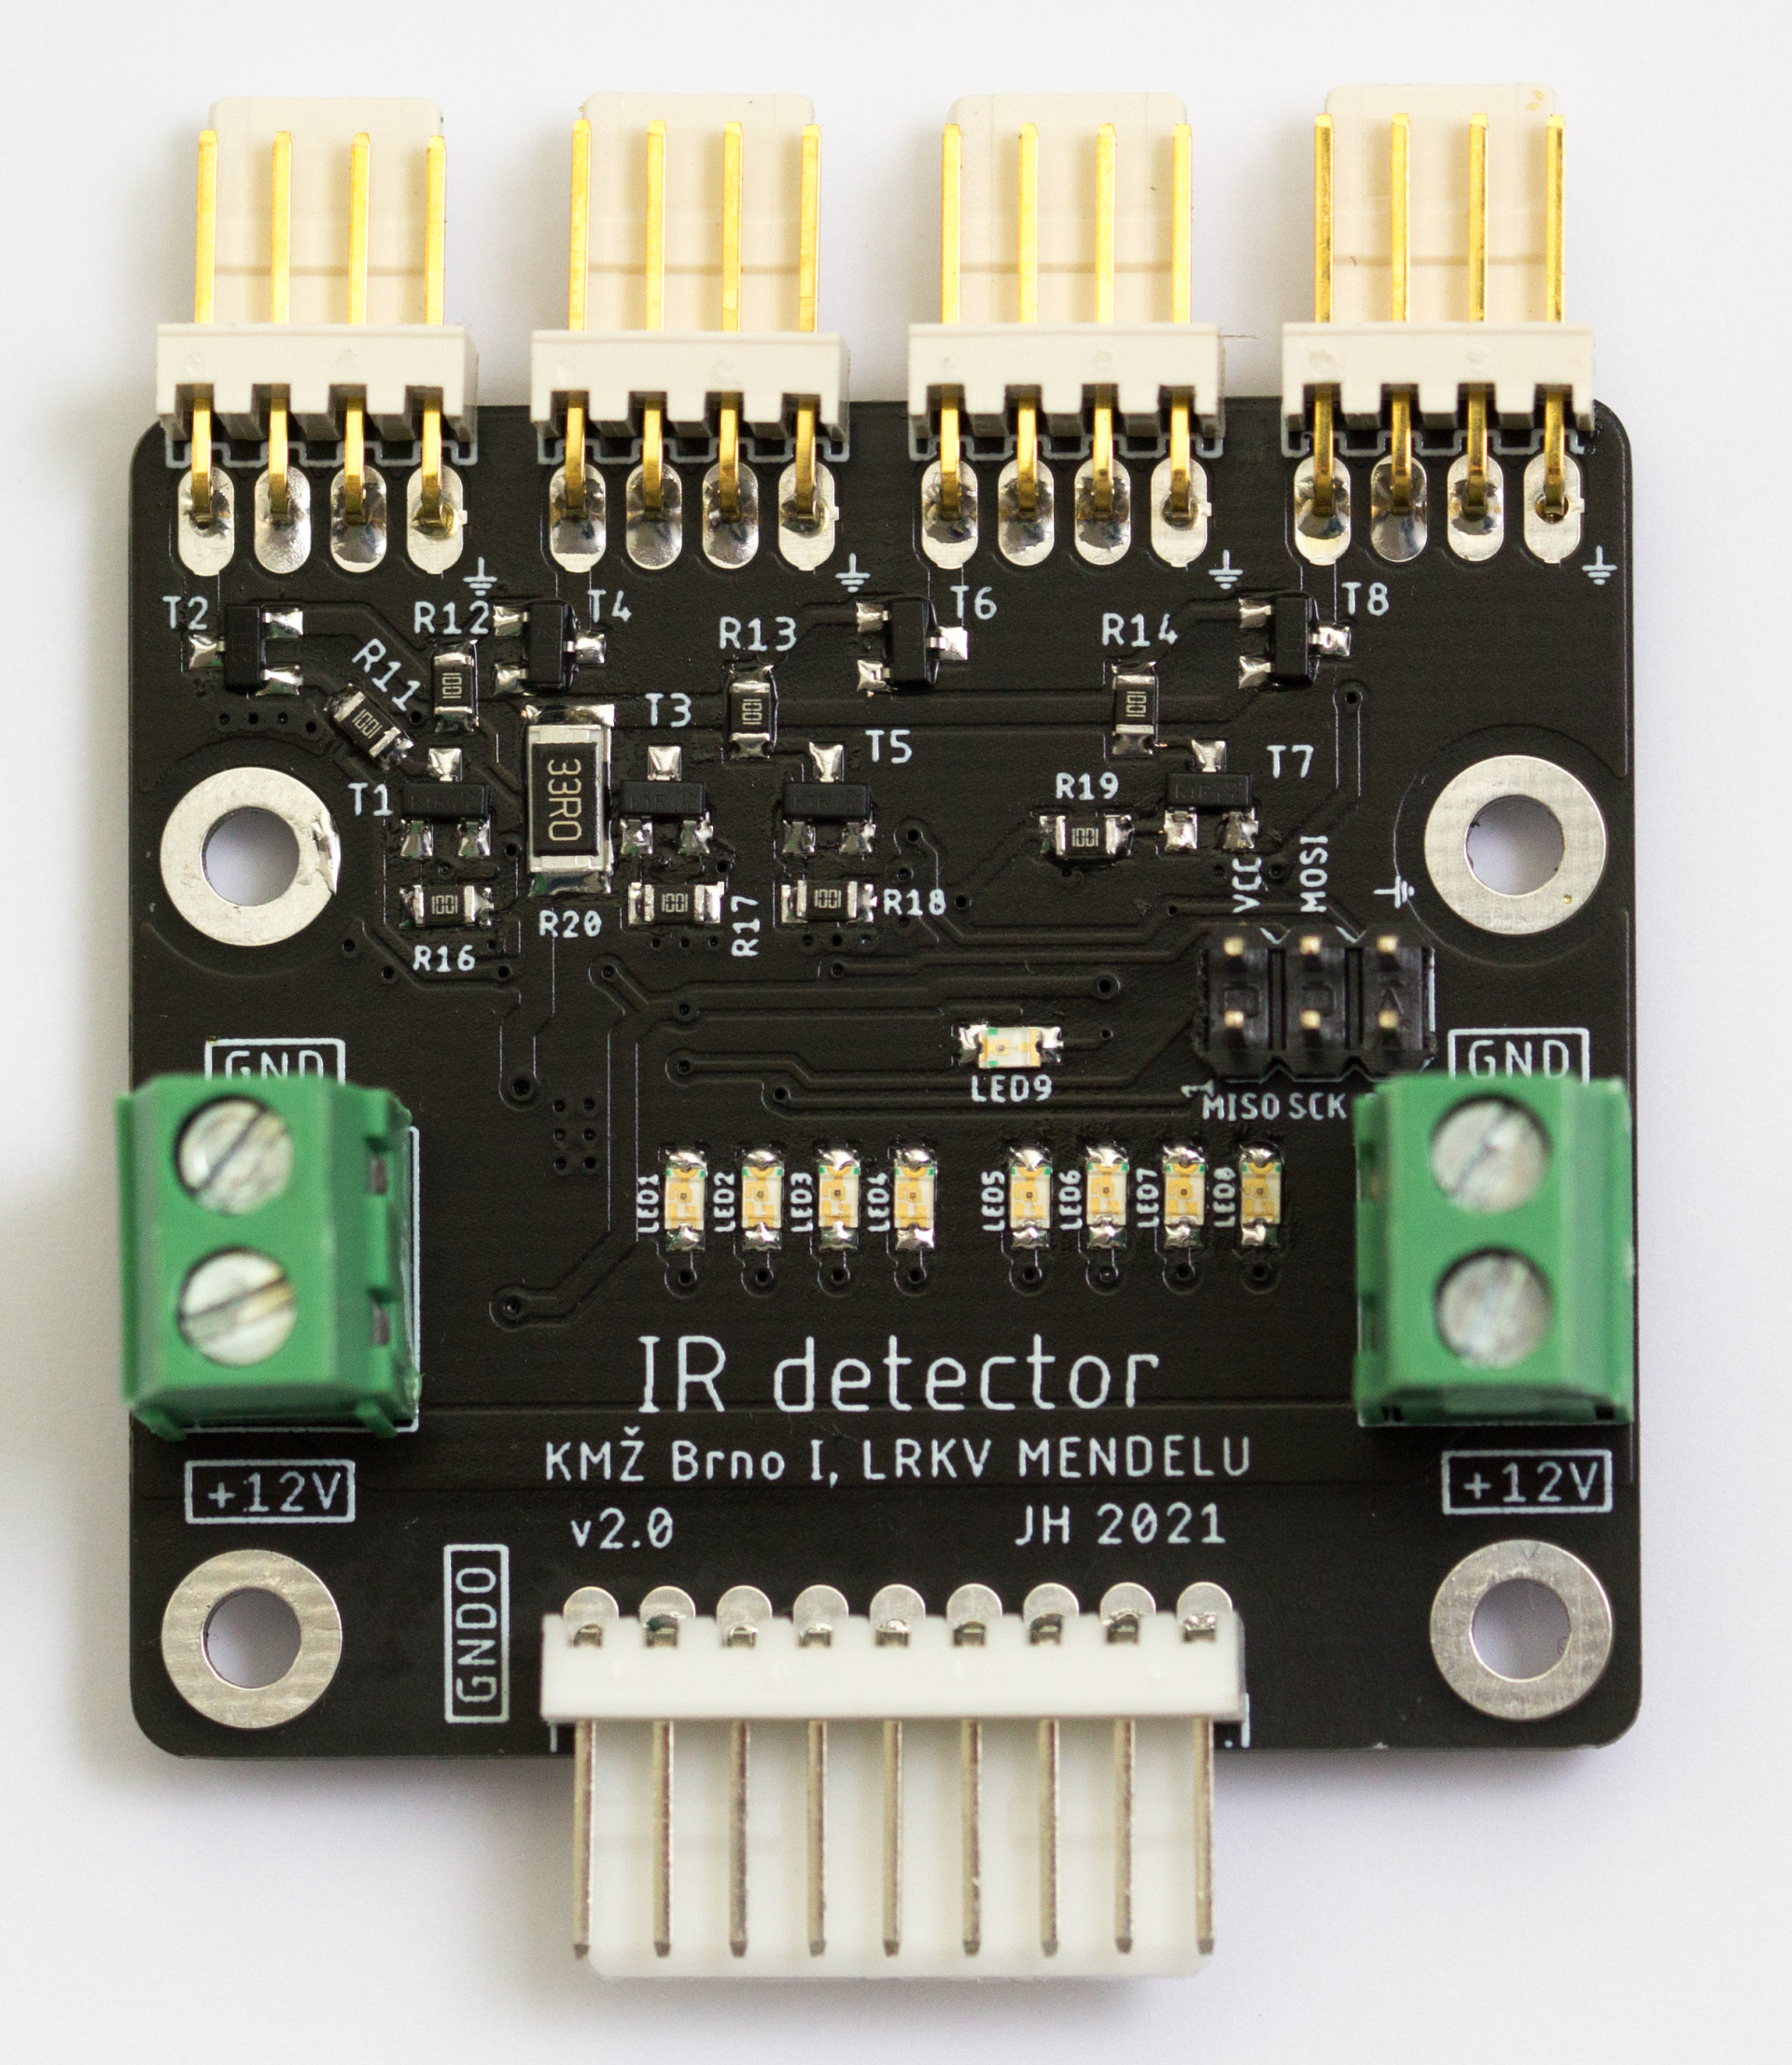
\includegraphics[width=0.5\textwidth]{data/irdet-front.jpg}}
\caption{Produkční verze desky IRdet}
\label{fig:irdet}
\end{figure}

Schéma zapojení a~\gls{dps} jsou k~dispozici jako open\-hard\-ware
projekt online\footnote{\url{https://github.com/kmzbrnoI/irdet-ele}}, firmware
je psán jako opensource projekt a je k~dispozici také
online\footnote{\url{https://github.com/kmzbrnoI/irdet-fw}}.
Schéma je dostupné v~příloze \ref{fig:irdet-sch}.

Hlavní komponentou návrhu je procesor řady \textit{Atmega8*}. Lze osadit
libovolný z~procesorů \textit{ATmega8a}, \textit{ATmega88}, \textit{ATmega328}
nebo jiný kompatibilní procesor. Signály z~fototranzistorů jsou zapojeny
v~režimu kapacitní vazby, viz \ref{fig:cap-bind}. Vysílací \gls{ir} diody jsou
buzeny přes tranzistory.  Proud do vysílacích diod je řízen omezovacím
rezistorem na stabilizovaném napětí.

Deska je navržena především z~\gls{smd} součástek (velikosti \textit{0805})
jako dvouvrstvá s~cílem osazovat součástky automaticky. Napájení desky se
očekává z~napájecího rozvodu \gls{mtb} modulů (ačkoliv to díky optickému
oddělení výstupů není nutné).
